\documentclass[t, screen, aspectratio=43]{beamer}
\usepackage[T1]{fontenc}
\usepackage[utf8]{inputenc}
\usepackage{epsf}
\usepackage{graphicx}

% Use the NTNU-temaet for beamer 
% \usetheme[style=ntnu|simple|vertical|horizontal, 
%     language=bm|nn|en, 
%     smalltitle, 
%     city=all|trondheim|alesund|gjovik]{ntnu2017}
\usetheme[style=helvet,language=en]{ntnu2017}

\usepackage[english]{babel}
\usepackage[style=numeric,backend=biber,natbib=false,sorting=none]{biblatex}

\title[Short title]{Ultra-Low Power PLL for Wake-up Radio Applications}
\subtitle{Specialization Project}
\author[C Nielsen]{Cole Nielsen}
\institute[NTNU]{Department of Electronic Systems, NTNU}
\date{27 August 2019}
%\date{} % To have an empty date

\addbibresource{example.bib} % Add bibliography database

% Set the reference style to numeric.
% See here: http://tex.stackexchange.com/questions/68080/beamer-bibliography-icon
\setbeamertemplate{bibliography item}[text] 

% Set bibliography fonts to a small size.
\renewcommand*{\bibfont}{\footnotesize}

\begin{document}

\begin{frame}
  \titlepage
\end{frame}

% Alternatively, special title page command to get a different background
% \ntnutitlepage

% #############################################################################
% Project objectives
% #############################################################################

\begin{frame}
  \frametitle{0Objective}
  \begin{block}{Broad goals}
    \begin{itemize}
      \footnotesize
      \item Design ultra-low-power frequency synthesizer to meet requirements for practical wake up receivers.
      \begin{itemize}
        \footnotesize
        \item \textbf{1 $\mu$W average consumption}
        \item Targeting 1\% duty cycle with 100 $\mu$W active power.
        \begin{itemize}
          \item Must be able to start and lock fast.
        \end{itemize}
      \end{itemize} 
      \item Sufficiently low phase noise for phase/frequency modulation schemes.
       \begin{itemize}
        \footnotesize
        \item Assume symbol of 2$\pi$ phase shift. 
        \item Allow for 250 kbps in 1 MHz OBW.\@
        \item Limits ICPM withing 1 MHz bandwidth to x degrees
      \end{itemize}      
      \item Target operation in 2.4 GHz ISM band.
    \end{itemize}
  \end{block}
\end{frame}

% #############################################################################
% Architecture - ideas
% #############################################################################

\begin{frame}
  \frametitle{Architecture}
  \begin{block}{Approach}
    \begin{itemize}
      \footnotesize
      \item Utilize digital PLL.\@ 
      \begin{itemize}
        \footnotesize
        \item Inherent feedback helps with PVT variation (yield).
        \item Calibration easy in digital design, agains help with PVT variation.
        \item Can store state when PLL in idle state, allowing for fast lock time.
      \end{itemize}       
      \item Utilize low duty cycle to achieve power     
      \begin{itemize}
        \footnotesize
        \item Can exploit semi-frequent calibration to improve performance.
        \item Possibly can run PLL open loop when lock is achieved to save power.
      \end{itemize} 
      \item Utilize oscillator running at 1/N subharmonic of target frequency.
      \begin{itemize}
        \footnotesize
        \item Use 2N phases in oscillator to achieve equivalent IQ sampling.
        \item Avoids having to run oscillator at 2x target frequency as done typically.
        \item 1/3 subharmonic operation should allow for dual mode 2.4G and 915M operation.
      \end{itemize} 
      \item Employ subsampling to reduce divider noise and TDC power?
    \end{itemize}
  \end{block}    

\end{frame}

% #############################################################################
% Architecture - block diagram
% #############################################################################

\begin{frame}
  \frametitle{Architecture}
  \begin{block}{Block Diagram}
    \center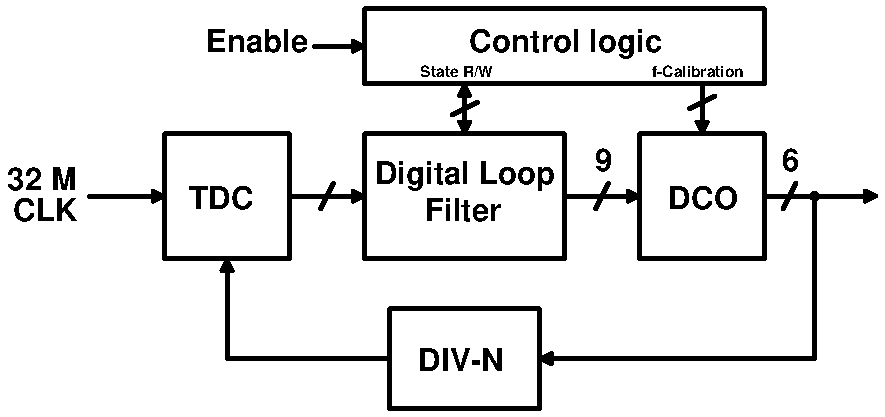
\includegraphics[width=0.8\textwidth, angle=0]{pll.pdf}
  \end{block}

\end{frame}

% #############################################################################
% Specs
% #############################################################################

\begin{frame}
  \frametitle{Architecture}
  \begin{block}{Specs}
    [table]
  \end{block}

\end{frame}

% #############################################################################
% Project phases slide 1
% #############################################################################

\begin{frame}
  \frametitle{Project Phases}
  \begin{block}{Autumn 2019}
    \footnotesize
    \begin{itemize}
      \item Finalize top-level architecture from requirements.
      \item System modeling and simulation.
      \begin{itemize}
        \footnotesize
        \item Determine requirements for TDC/DCO/Divider/logic (bits of resolution, accuracy etc) to meet PLL performance specifications.
        \item Determine digital logic for loop filter, validate stability and lock time performance.
      \end{itemize}
      \item Translate component-level specifications to circuit designs.
      \begin{itemize}
        \footnotesize
        \item Research what works.
        \item Try, fail, try again until functional at schematic level.
        \begin{itemize}
          \footnotesize
          \item I expect the TDC to be difficult.
      \end{itemize}
      \end{itemize}      
    \end{itemize}
  \end{block}
\end{frame}

% #############################################################################
% Project phases slide 2
% #############################################################################


\begin{frame}
  \frametitle{Project Phases (continued)}
  \begin{block}{Spring 2020}
    \begin{itemize}
      \footnotesize
      \item Layout
      \item Characterization
    \end{itemize}
  \end{block}
\end{frame}


\begin{frame}
  \frametitle{References}
  \printbibliography
\end{frame}

\end{document}
